
The character classifier classifies images with handwritten characters as described in section~\ref{sec:overview_of_classifiers}. A sequence of observation symbols is extracted from the images given as training data and when an image shall be classified. This process is called feature extraction. 

    \begin{figure}[htb] 
      \begin{center}
	\leavevmode
	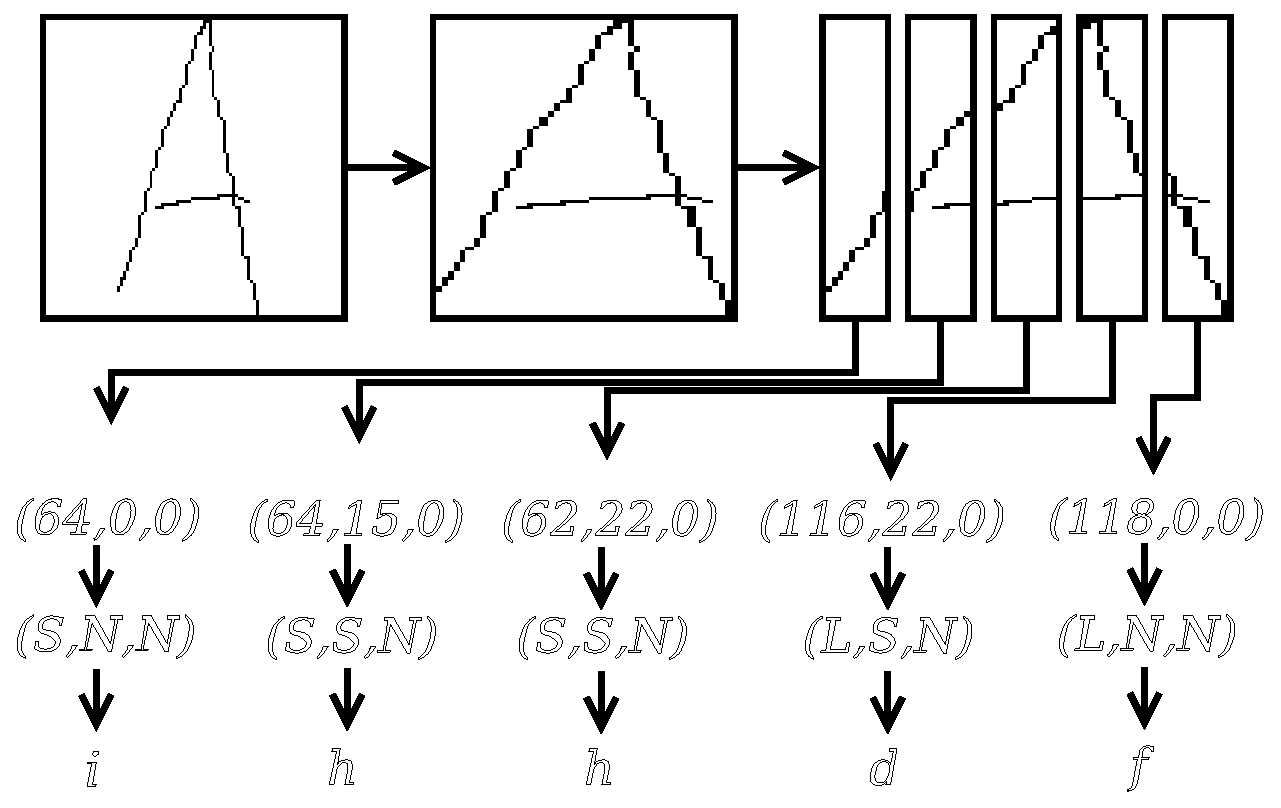
\includegraphics[width=110mm]{image_feature_extraction.eps}%width=115mm,height=40mm
      \end{center}
      \caption{Example of image feature extraction.}
      \label{fig:image_feature_extraction}
    \end{figure}

As mentioned in section~\ref{sec:problem}, our system assume that there is one image per character, that the lines in the characters are of a single color and the width of the lines is one. The feature extraction process can be divided into the following steps:

\begin{enumerate}
  \item The scaling step makes sure that the character fills the whole image. Because of this step, it does not matter where in the given image the character is painted. The scaling may have the problem that the lines are getting thicker than one pixel after scaling if the original painted character just fills a small part of the image\footnote{The standard Java image scaling algorithm is used for the scaling.}. This problem will be handled in some sense if the training examples contains images where the character fills a small part of the image. The following algorithm is used to do the scaling:
  \begin{enumerate}
    \item The minimum rectangle $R$ in the image that contains the whole character is found.
    \item The rectangle $R$ is scaled to fill the size of the original image. The scaled version of $R$ is returned as the scaled image.
  \end{enumerate}
  \item The new scaled image is sliced into $N$ vertical segments of the same since.
  \item An observation symbol is extracted from every segment in the following way:
  \begin{enumerate}
    \item The number of pixels in the three largest components in the segment are found and put into a triple $(s_{1},s_{2},s_{3})$ which is sorted so the largest number is first. A component is defined as a set of colored pixels that are connected and that contains all pixels that are connected to one of the pixels in the set. Two colored pixels are connected if they are neighbors or if it is possible two create a path of colored connected pixels between them. All pixels except the border pixels have 8 neighbors. If the segment contains less than three components, the triple is filled with zeros.
    \item The elements in the triple is classified to be $Large$, $Small$ or $None$. The classification function $c$ is defined as in equation~\ref{eq:classification_function}.
    \begin{equation}\label{eq:classification_function}
    c(s) = None \text{ if } s = 0, Large \text{ if } s > d \text{ and } Small \text{ otherwise}
    \end{equation}, where $d$ is a classification constant. The triple $(s_{1},s_{2},s_{3})$ is translated to a triple of classes $(c_{1},c_{2},c_{3})$ by applying the function $c$ to all elements in the triple.
    \item The triple of classes is mapped to an observation symbol. The mapping is defined by the set of relations that can be found in equation~\ref{eq:class_triple_to_observation_symbol_mappings}.

    \begin{equation}\label{eq:class_triple_to_observation_symbol_mappings}
     \substack{ LLL\rightarrow a,LLS\rightarrow b,LSS\rightarrow c,LSN\rightarrow d,LLN\rightarrow e,LNN\rightarrow f,\\
    SSS\rightarrow g,SSN\rightarrow h,SNN\rightarrow i,NNN,\rightarrow j }
    \end{equation}
    , where $LSN$ is a short form of $(Large,Small,None)$ and so on.
  \end{enumerate}  
\end{enumerate}

The classification constant $c$ and the number of segments $N$ are parameters to the feature extractor. An example of feature extraction for an image can be seen in figure~\ref{fig:image_feature_extraction}.